In this section we present a method to derive concurrency oracles from the instruction
semantics encoded in the  metalanguage (definition~\ref{def:metalanguage}).
More specifically, we are aiming to reason about instructions,
which have only~\emph{static} dependencies.

Let us now introduce the formal definitions and Haskell encodings of the concepts
required for building concurrent oracles.

First of all we need to defined the notions of input and output dependencies of
a computation.

\textbf{Definition (input dependency):\label{def:in-dependencies}}
Consider a term $f$ of an applicative metalanguage~\hs{Semantics Applicative a}. A key $k$
is an~\textbf{input dependency} of the term $f$ if the term $f$
performs a~\textbf{read} of the key $k$.

\textbf{Definition (output dependency):\label{def:out-dependencies}}
Consider a term $f$ of an applicative metalanguage~\hs{Semantics Applicative a}. A key $k$is
an~\textbf{output dependency} of the term $f$ if the term $f$
performs a~\textbf{write} of the key $k$.

\textbf{Definition (dependency):\label{def:dependencies}}
Consider a term $f$ of an applicative metalanguage~\hs{Semantics Applicative a}.
The~\textbf{dependencies} of the term $f$ are a pair of sets $I$ and $O$,
comprising the input and output dependencies of the term $f$, respectively.

In the Haskell implementation, we do not distinguish between input and output dependencies
in the type level, thus the function determining the dependencies of a computation
has the following type:

\begin{minted}{haskell}
dependencies :: Semantics Applicative a -> Maybe ([Key], [Key])
\end{minted}

The~\hs{Maybe} type constructor comes from the definition of the metalanguage:
if a computation is faulty (returns~\hs{Nothing}) it is impossible to extract
its static dependencies. Successful static analysis yields a pair of lists representing
the sets of input and output dependencies of a computation.

To extract the static data dependencies of an applicative computation we need to
interpret its semantics in a special context, which needs a bit of an additional
explanation.

\newpage

\subsection{The constant functor}

The~\hs{Const a b} data type is defined as follows:

\begin{minted}{haskell}
newtype Const a b = Const { getConst :: a }
\end{minted}

A value of the~\hs{Const a b} is just a value of any type~\hs{a}
wrapped in a data constructor. However, it is important that the type constructor
has a~\emph{phantom type} variable. This type variable gives a possibility to
declare useful instances of standard Haskell type classes such as~\hs{Functor},
\hs{Applicative} and \hs{Monad} for \hs{Const a}. We would like to use this
datatype as a computational context for applicative semantics, hence we declare
the corresponding instance\footnote{\hs{Const a} must also be declared an instance
of~\hs{Functor}, where~\hs{fmap _ (Const v) = Const v}}:

\begin{minted}{haskell}
instance Monoid m => Applicative (Const m) where
    pure _              = Const mempty
    Const f <*> Const v = Const (f `mappend` v)
\end{minted}

This instance exactly describes the desired behaviour of static dependency tracking
computational context.~\hs{Const [Key]} is an applicative functor that ignores
its enclosed value, but accumulates the declared dependencies using the~\hs{Monoid}
instance for Haskell list data type\footnote{The empty list~\hs{[]} is the
neutral element and the list concatenation~\hs{(++)} is the associative binary operation}.

\subsection{Dependencies}

Using the elegant~\hs{Const a b} abstraction we define the \hs{dependencies} function:

\begin{minted}{haskell}
dependencies :: Semantics Applicative a
             -> Maybe ([Key], [Key])
dependencies task =
    partitionEithers . getConst <$>
    task trackingRead trackingWrite
  where trackingRead  k    =       Const [Left k]
        trackingWrite k fv = fv *> Const [Right k]
\end{minted}

It instantiate the metalanguage combinators with computations in the tracking read
and write functions. In fact, \hs{trackingRead} does not perform any reading and just tracks
the key as an input dependency, whereas \hs{trackingRead} tracks its key as
an output dependency and executes the effectful computation \hs{fv}, which is
in fact a call of \hs{trackingRead}. The resulting list of keys gets unwrapped and
unzipped.

Now we are ready to define concurrency oracles for terms of the
applicative metalanguage.

\newpage
\subsection{Concurrency oracle}
% \vspace{-2em}
A concurrency oracle is a function taking two computations and statically
determining if they are data~\emph{concurrent}, i.e. do not share any
data dependencies.


\textbf{Definition (concurrency status):\label{def:concurrency-status}}
% \vspace{-3em}
\begin{minted}{haskell}
data ConcurrencyStatus k = Concurrent
                         | ReadConflict      [k]
                         | WriteConflict     [k]
                         | ReadWriteConflict [k] [k]
\end{minted}
% \vspace{-3em}

\noindent Two terms of the metalanguage are concurrent if they do not share any data dependencies.
The have a read or write conflict if they share any input or output dependencies,
respectively. If the share both input and output dependencies then they are considered to
have a read-write conflict. The definition of a concurrency oracle closely resembles
this specification:

\textbf{Definition (concurrency oracle):\label{def:oracle}}
Consider a term $f$ and $g$ of an applicative metalanguage~\hs{Semantics Applicative a}.
A~\emph{concurrency oracle} is defined as a Haskell function
% \vspace{-3em}
\begin{minted}{haskell}
concurrencyOracle :: Semantics Applicative k v1 a
                  -> Semantics Applicative k v2 a
                  -> Maybe (ConcurrencyStatus k)
concurrencyOracle p q = do
    (pIns, pOuts) <- dependencies p
    (qIns, qOuts) <- dependencies q
    let readConflicts  = intersect pIns qIns
        writeConflicts = intersect pOuts qOuts
    pure $ case (readConflicts, writeConflicts ) of
                ([], []) -> Concurrent
                (rs, []) -> ReadConflict rs
                ([], ws) -> WriteConflict ws
                (rs, ws) -> ReadWriteConflict rs ws

\end{minted}
% \vspace{-3em}
In order to determine the concurrency status between two terms, the oracle
retrieves their static dependencies and performs a pattern-matching in the
set intersections.

Let us now present two examples to illustrate the usage of concurrency
oracles.

\subsection{Example oracles}

Two load instruction with different arguments are indeed concurrent:

\begin{minted}{haskell}
ghci> concurrencyOracle (semanticsA (Load R0 0))
                        (semanticsA (Load R1 1))
Just Concurrent
\end{minted}

\begin{minipage}{0.55\textwidth}
Extending the first computation with an addition instruction causes a read conflict:
\begin{minted}{haskell}
ghci> let p1 = blockSemanticsA [ Load R0 0
                               , Add  R0 1 ]
ghci> let p2 = semanticsA (Load R1 1))
ghci> concurrencyOracle
Just (ReadConflict [Addr 1])
\end{minted}
We can produce a graphical
representation of dependencies between and
within computations\hs{p1} and \hs{p2} with
the following commands:
\begin{minted}{haskell}
ghci> let g1 = programDataGraph
          (zip [0..] [Load R0 0, Add R0 1])
ghci> let g2 = programDataGraph
               (zip [0..] [Load R1 1])
ghci> drawGraph (overlay g1 g2)
\end{minted}
\end{minipage}%
\hfill
\begin{minipage}{0.35\textwidth}
\begin{figure}[H]
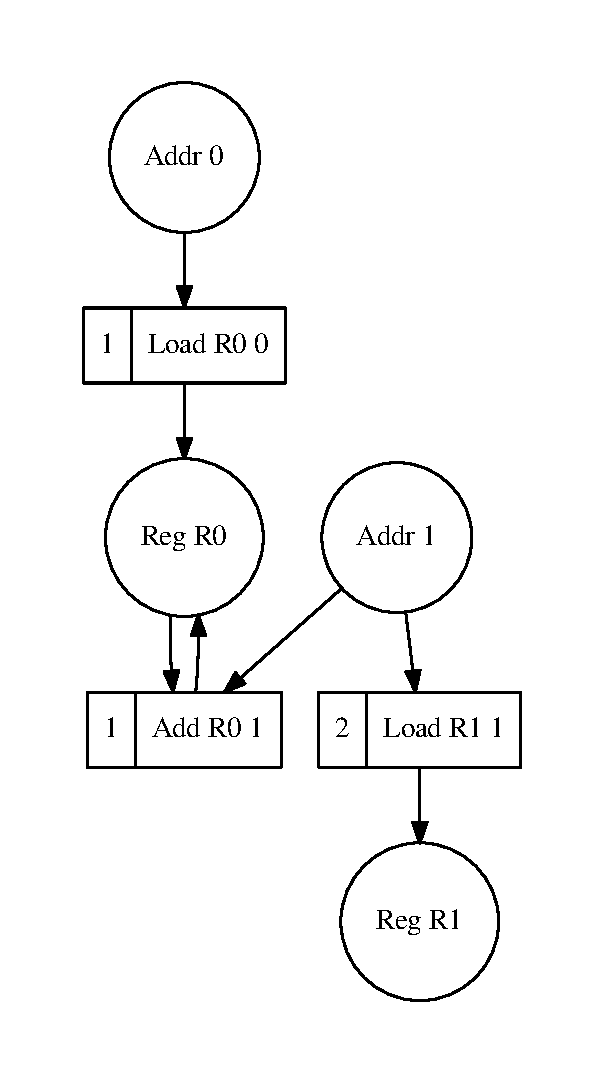
\includegraphics[width=20em]{img/oracle2.pdf}
\end{figure}
\end{minipage}%

\noindent In the graph, instructions labelled with 1 and 2 belong to the blocks~\hs{p1}
and~\hs{p2} respectively. Both computations share the register
\texttt{R0}, just like the oracle has foreseen.
